\documentclass{article}

\usepackage[a4paper,hmargin=1.2in,vmargin=1.5in]{geometry}
\usepackage[parfill]{parskip} % for distance between paragraphs
\usepackage{ragged2e} % for alignment
\usepackage{hyperref} % for link
\usepackage{fancyhdr} % for header, footer
\usepackage{xcolor}  % for color
\usepackage{graphicx} % for figure
\usepackage{subcaption}
\usepackage{floatrow} % for formatting figures
\usepackage{enumitem} % for adjusting list spacing 
\usepackage{amsmath} 
\usepackage{amsthm} 
\usepackage{amssymb} 
\usepackage{esint}

\newtheorem{theorem}{Theorem}
\newtheorem{lemma}{Lemma}
\newtheorem{corollary}[theorem]{Corollary}
\newtheorem{proposition}{Proposition}[section]
\theoremstyle{remark}
\newtheorem*{remark}{Remark}

\setlength{\parskip}{0.5em}

\pagestyle{fancy}
\fancyhf{}
\lhead{190050113-190050080-190020010}
\rhead{CS 215}
\cfoot{Page \thepage}
\renewcommand{\footrulewidth}{1pt}

\usepackage{titlesec}
\titleformat{\section}
  {\Large\bfseries}{}{1em}{}

\title{Assignment 1: CS 215}

\author{
  \textbf{190050113} Shivam Raj
  \and
  \textbf{190050080} Pawan Kumar
  \and
  \textbf{190020010} Aman Singh
}

\date{September 14, 2020}

\begin{document}

\pagenumbering{gobble}
\maketitle
\tableofcontents

% \newpage
\pagenumbering{arabic}

\section{Question 1}
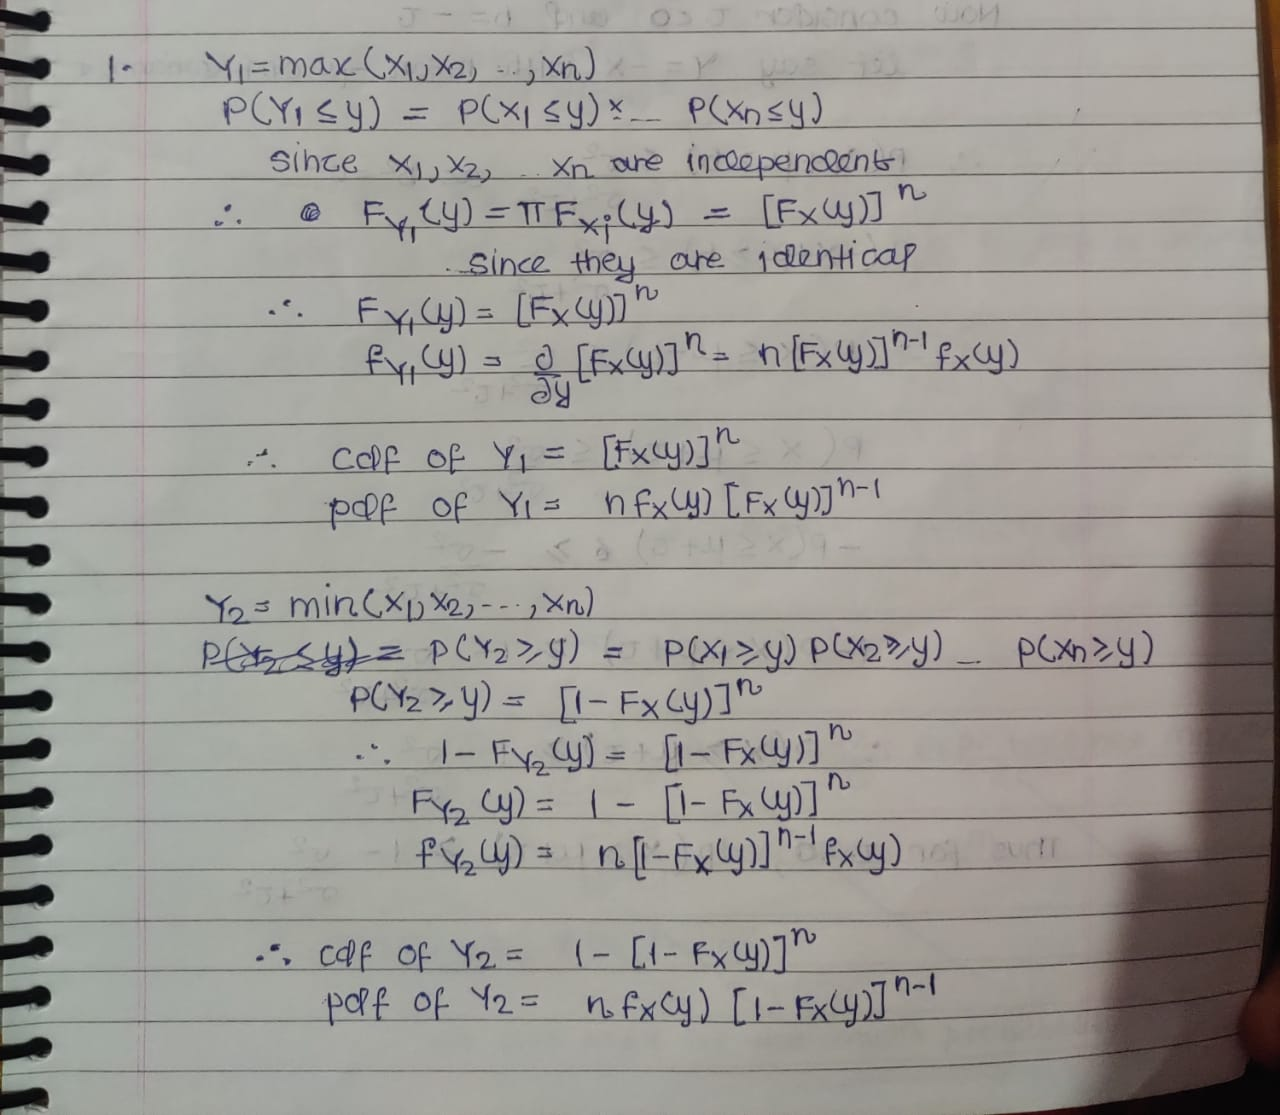
\includegraphics[width=\textwidth, height=\textheight, keepaspectratio]{1.jpeg} \par
\section{Question 2}

\section{Question 3}
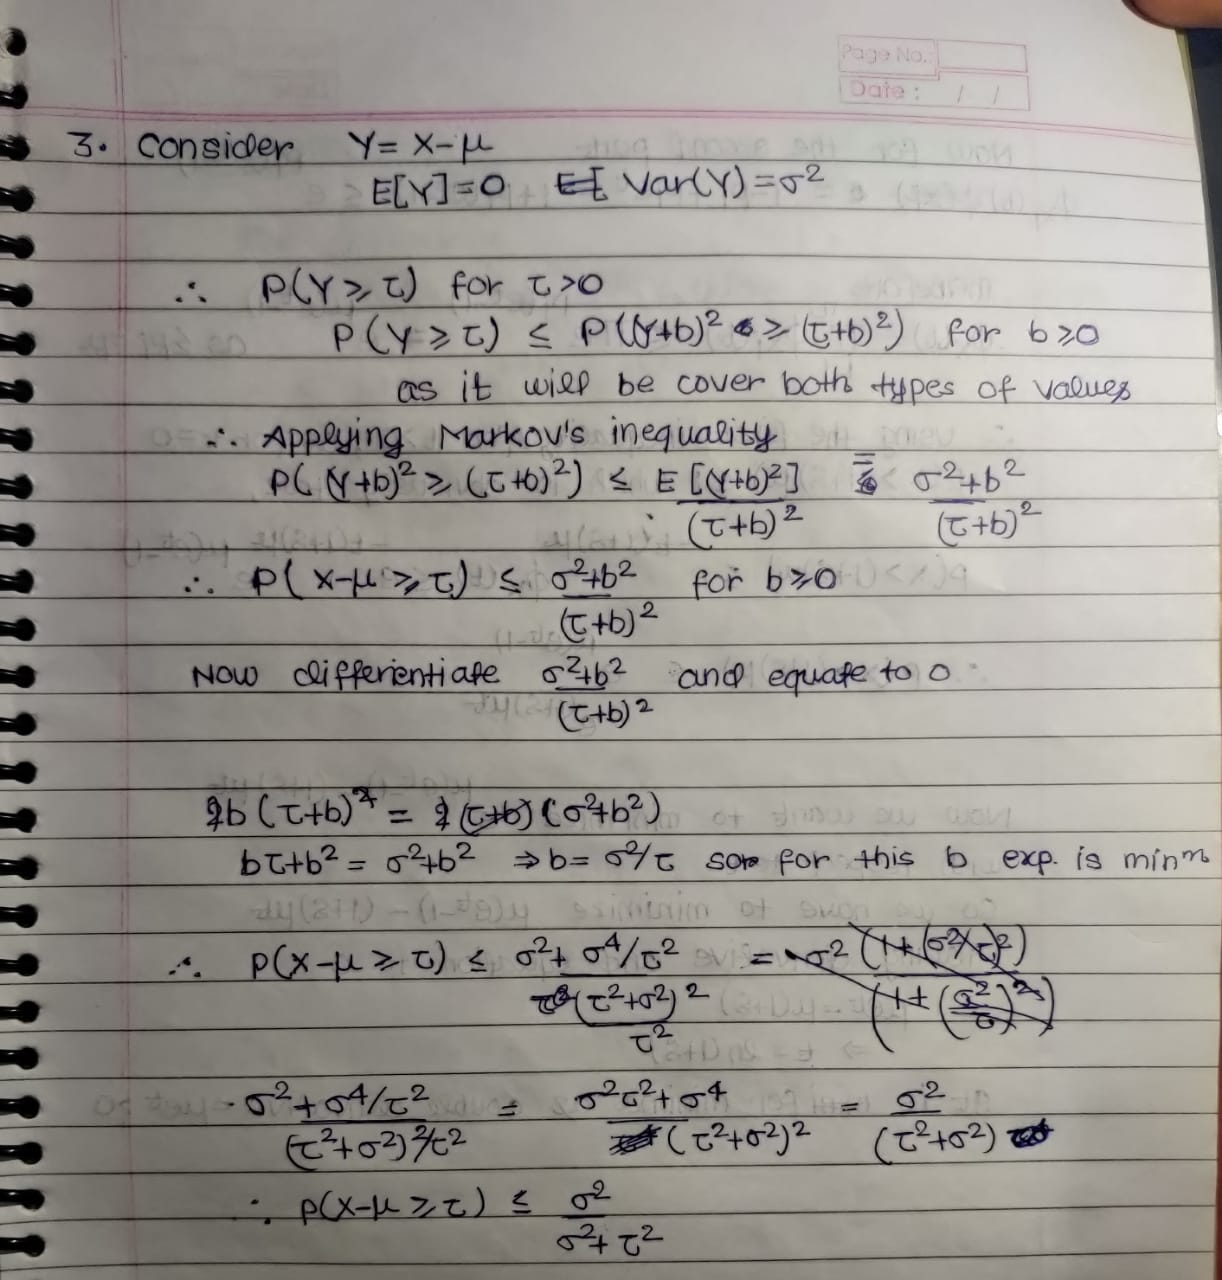
\includegraphics[width=\textwidth, height=\textheight, keepaspectratio]{3a.jpeg} \par
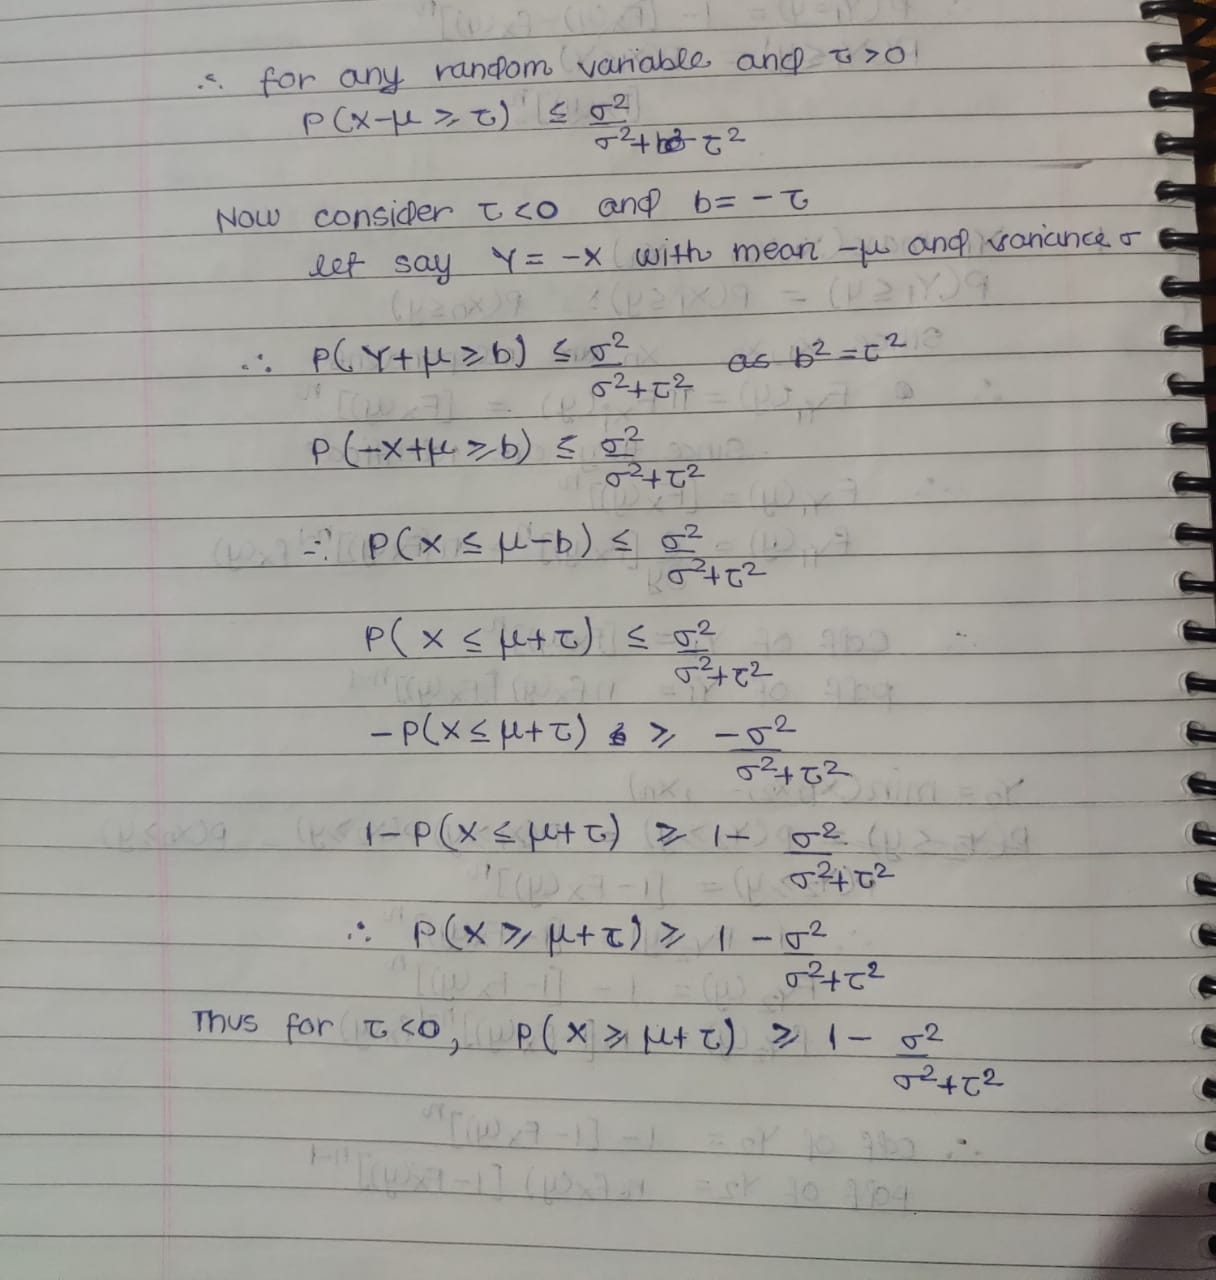
\includegraphics[width=\textwidth, height=\textheight, keepaspectratio]{3b.jpeg}\par
\section{Question 4}
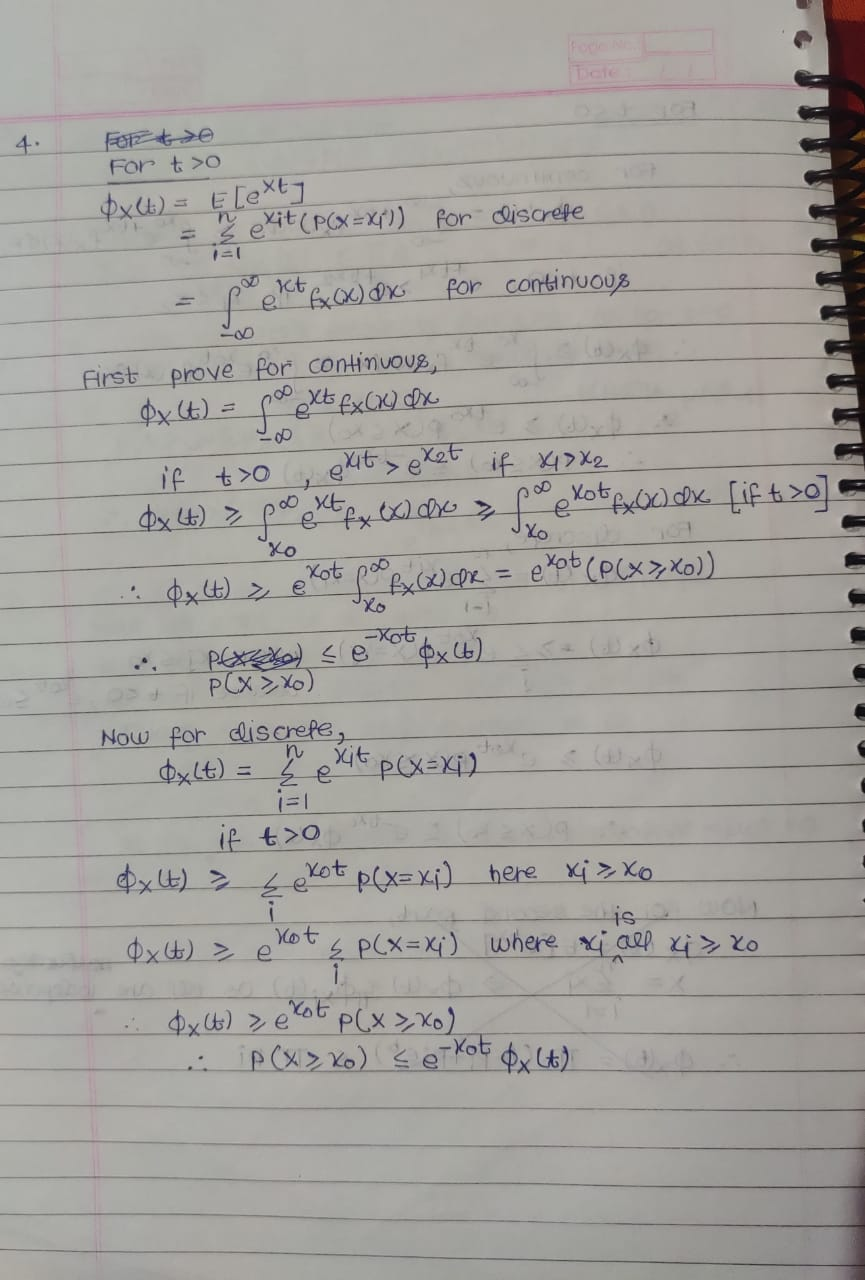
\includegraphics[width=\textwidth, height=\textheight, keepaspectratio]{4a.jpeg} \par
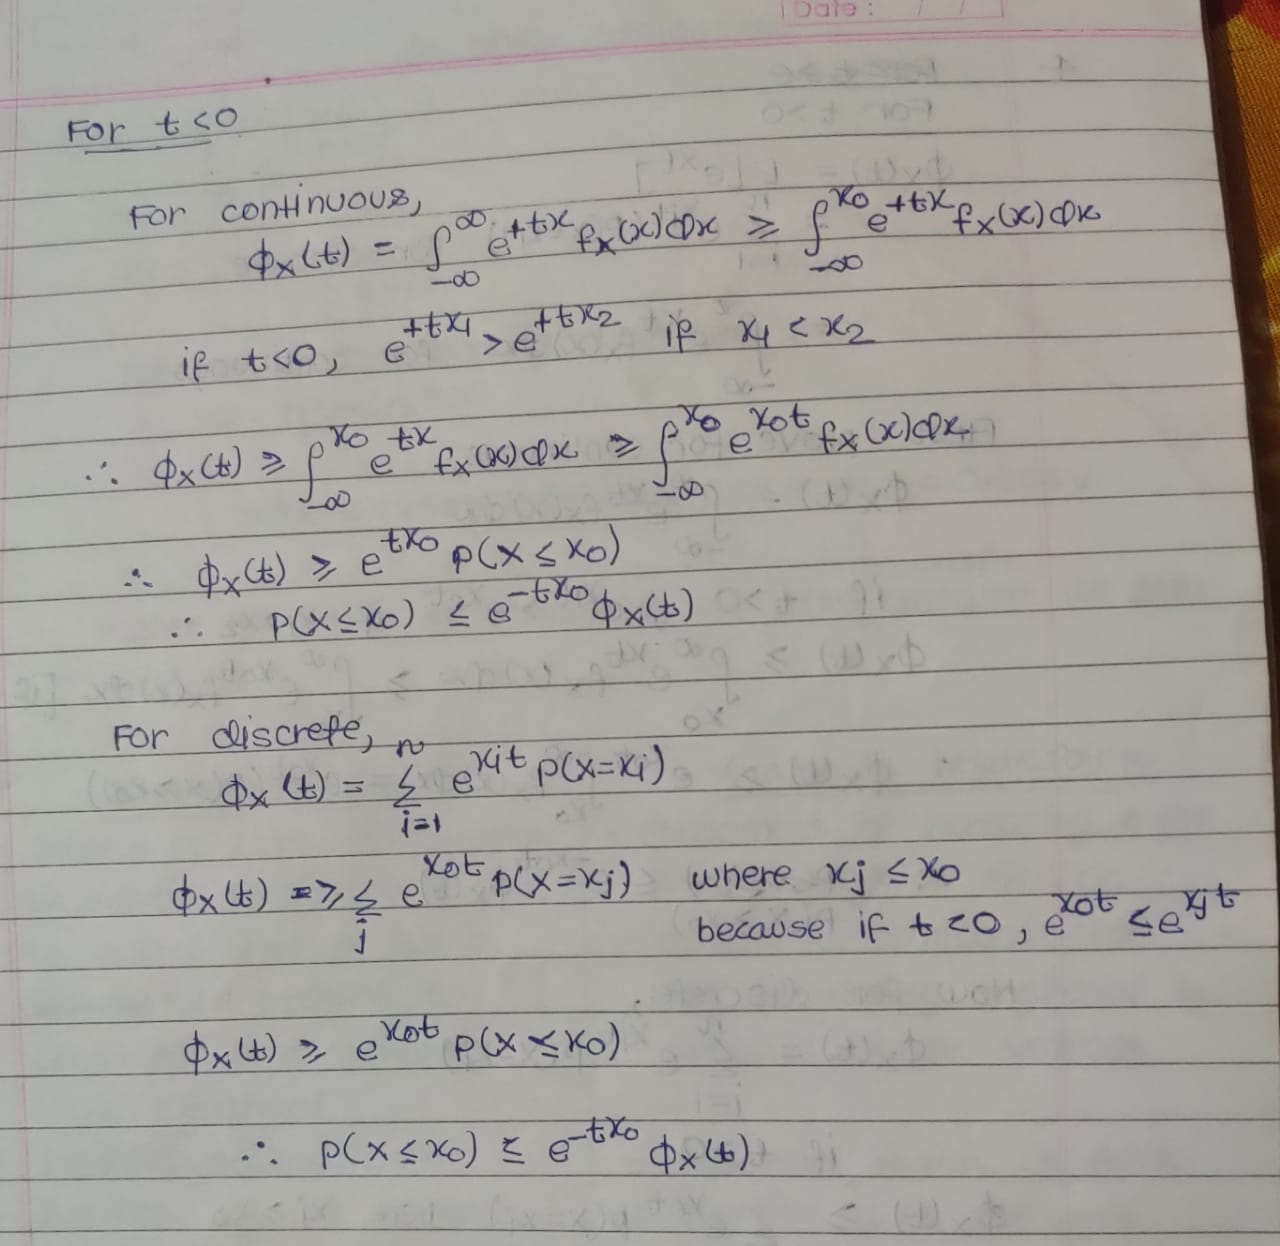
\includegraphics[width=\textwidth, height=\textheight, keepaspectratio]{4b.jpeg} \par
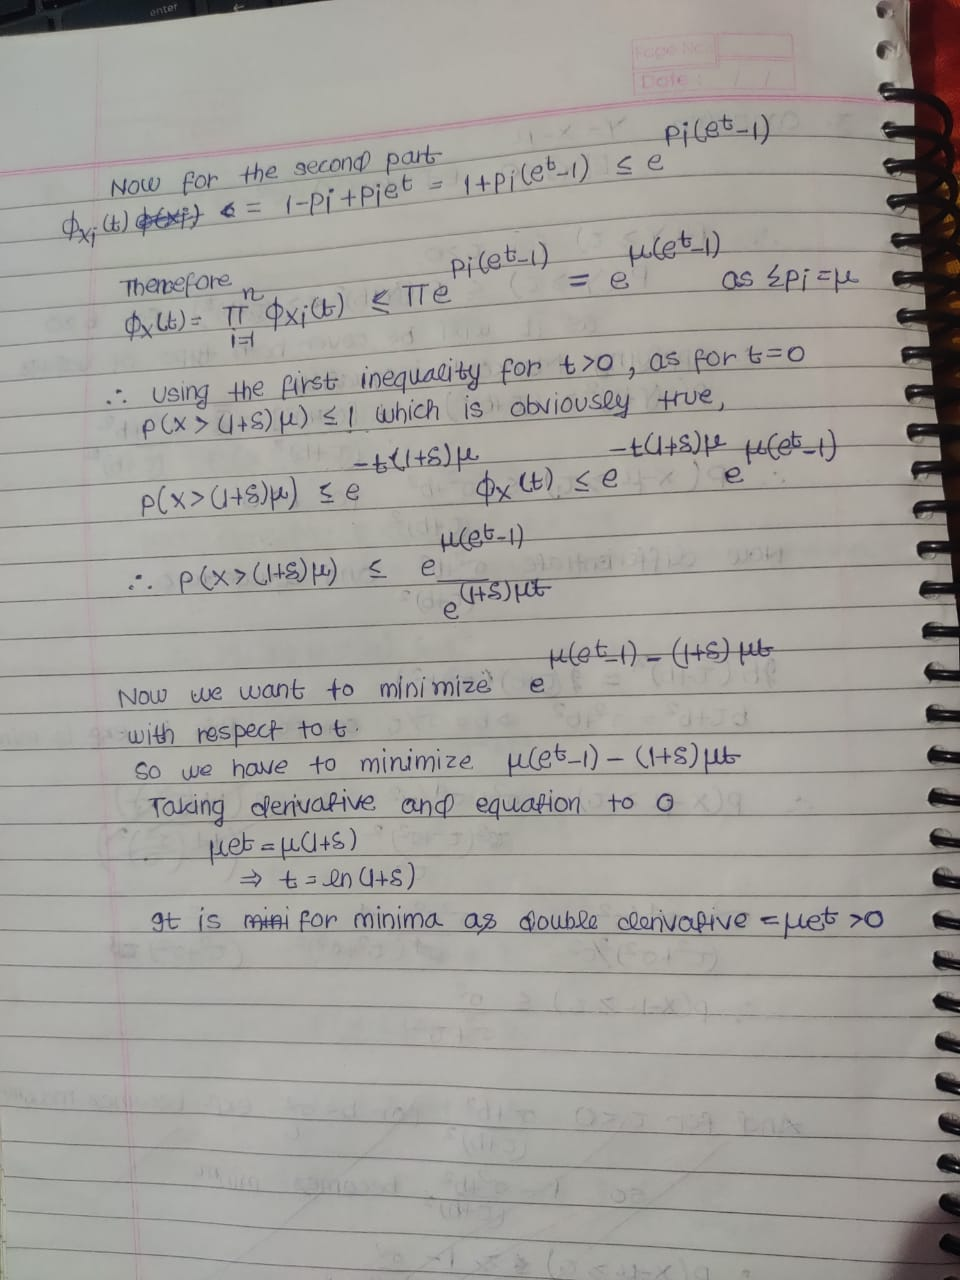
\includegraphics[width=\textwidth, height=\textheight, keepaspectratio]{4c.jpeg} \par
\newpage
\section{Question 5}
Code for this qsn is in file named 'q5.m' \par
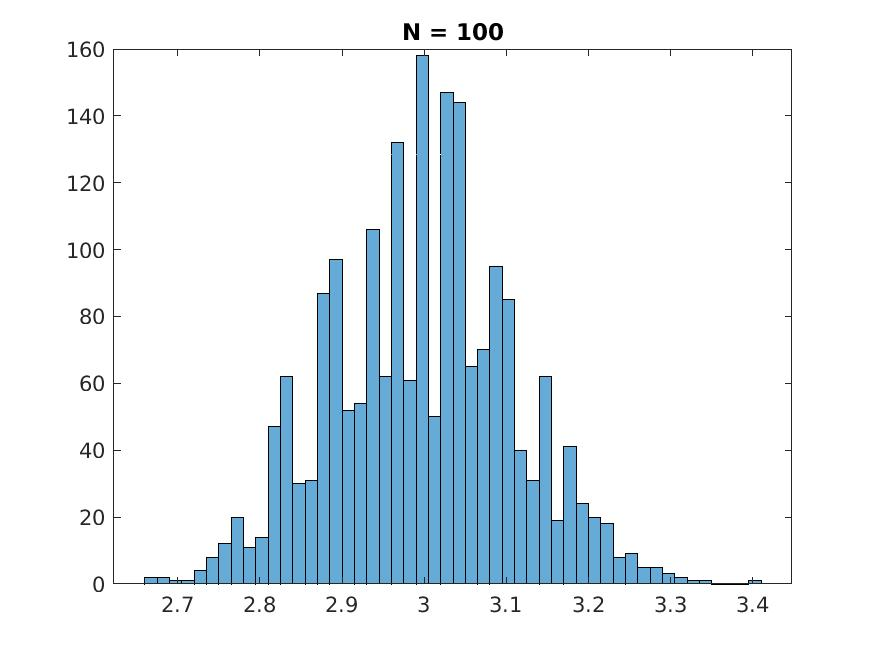
\includegraphics[width=\textwidth, height=\textheight, keepaspectratio]{p1_100.jpg}\par
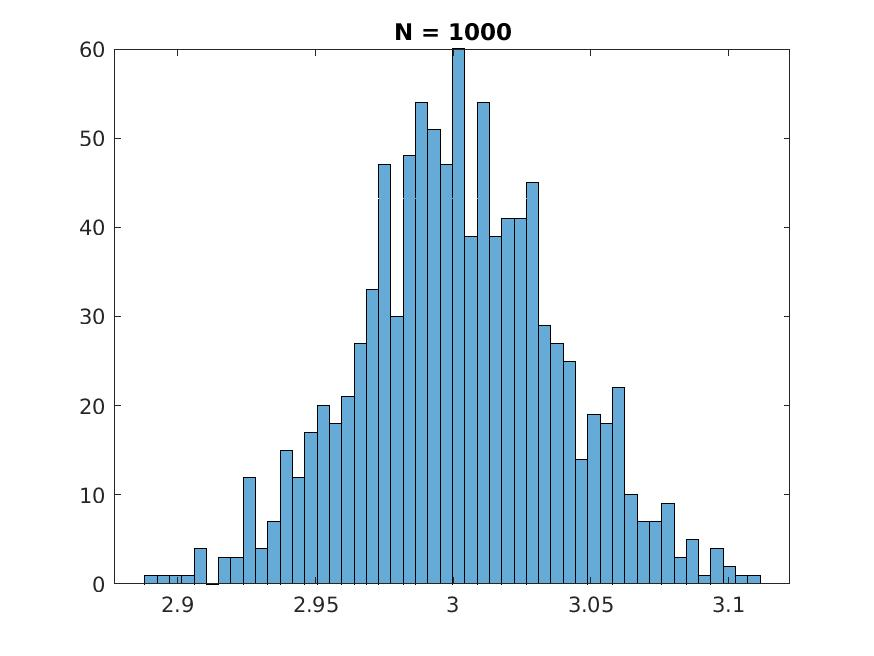
\includegraphics[width=\textwidth, height=\textheight, keepaspectratio]{p1_1000.jpg}\par
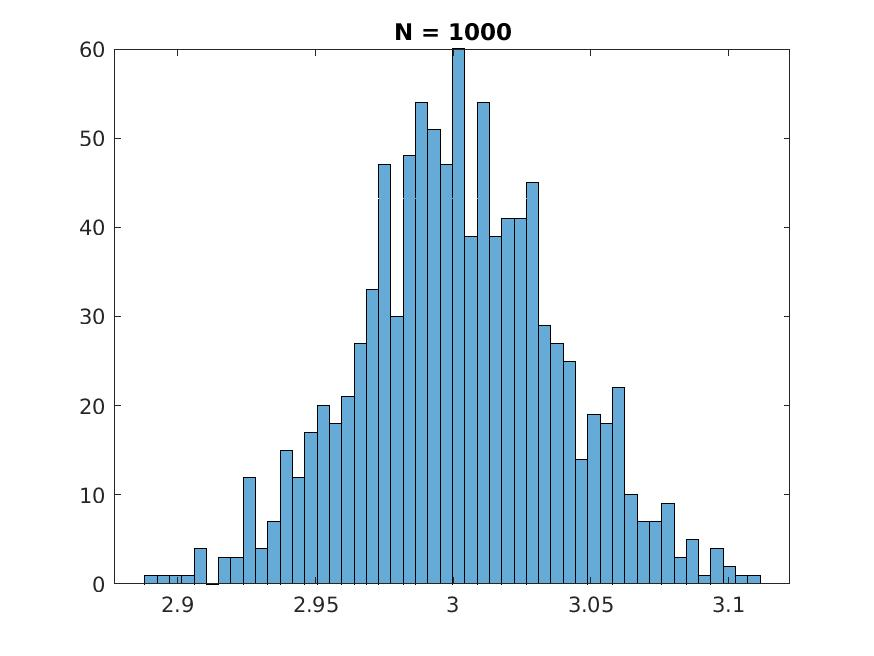
\includegraphics[width=\textwidth, height=\textheight, keepaspectratio]{p1_1000.jpg}\par
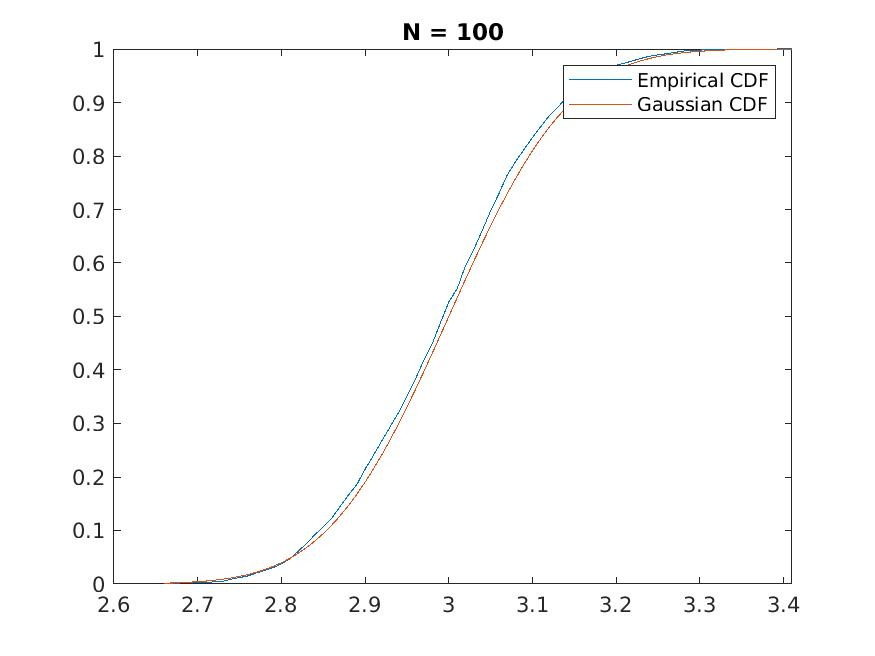
\includegraphics[width=\textwidth, height=\textheight, keepaspectratio]{p2_100.jpg}\par
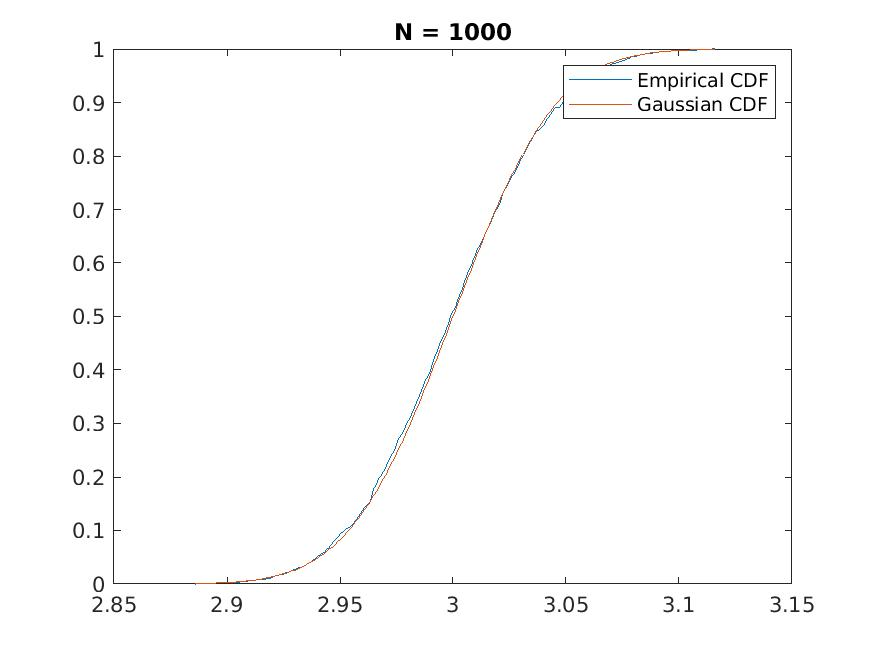
\includegraphics[width=\textwidth, height=\textheight, keepaspectratio]{p2_1000.jpg}\par
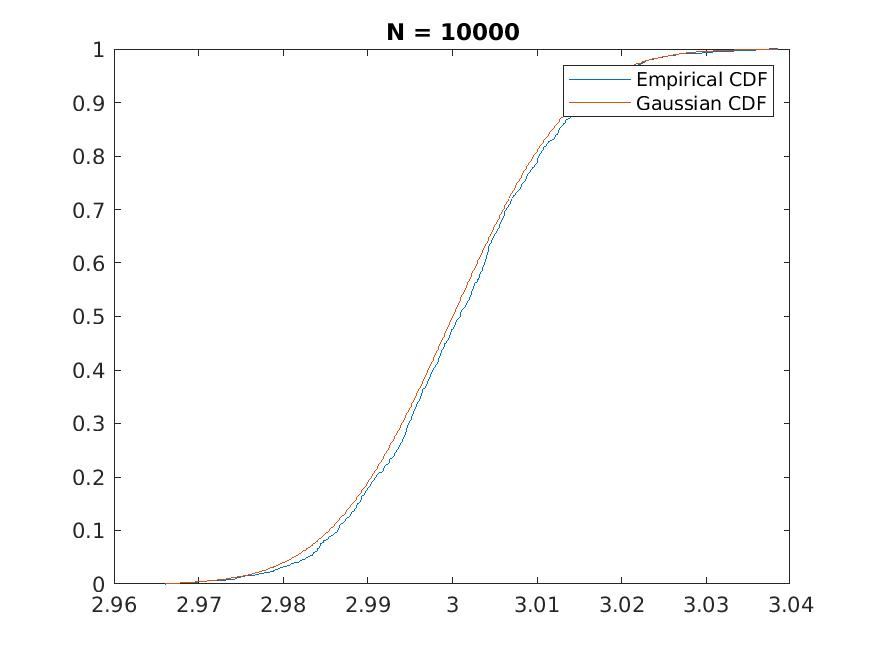
\includegraphics[width=\textwidth, height=\textheight, keepaspectratio]{p2_10000.jpg}\par
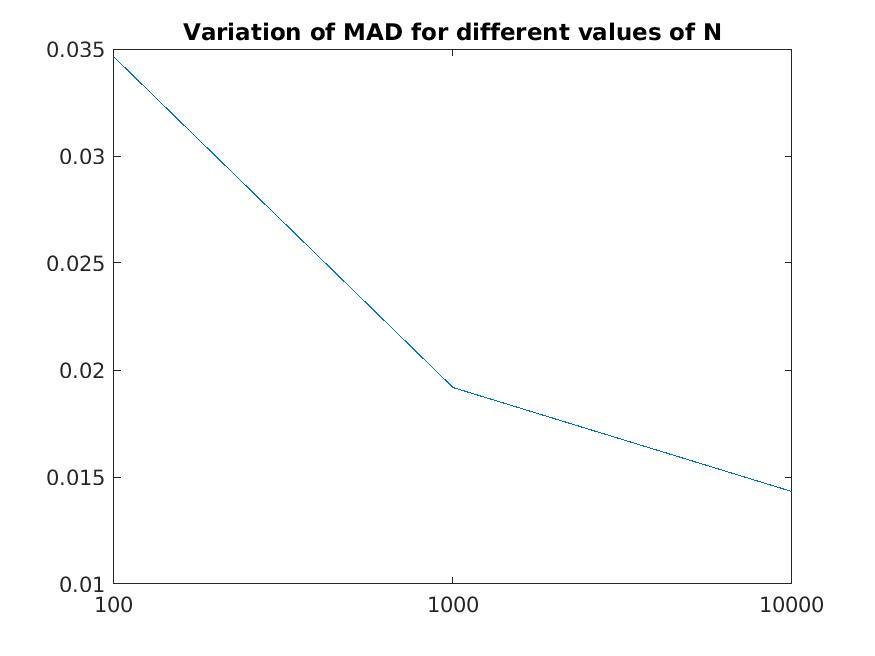
\includegraphics[width=\textwidth, height=\textheight, keepaspectratio]{p3.jpg}\par
\newpage
\section{Question 6}
Code of this question is in the file 'q6.m' \par
% \begin{figure} [h!]
% \centering
% \begin{subfigure}[b]{0.4\linewidth}
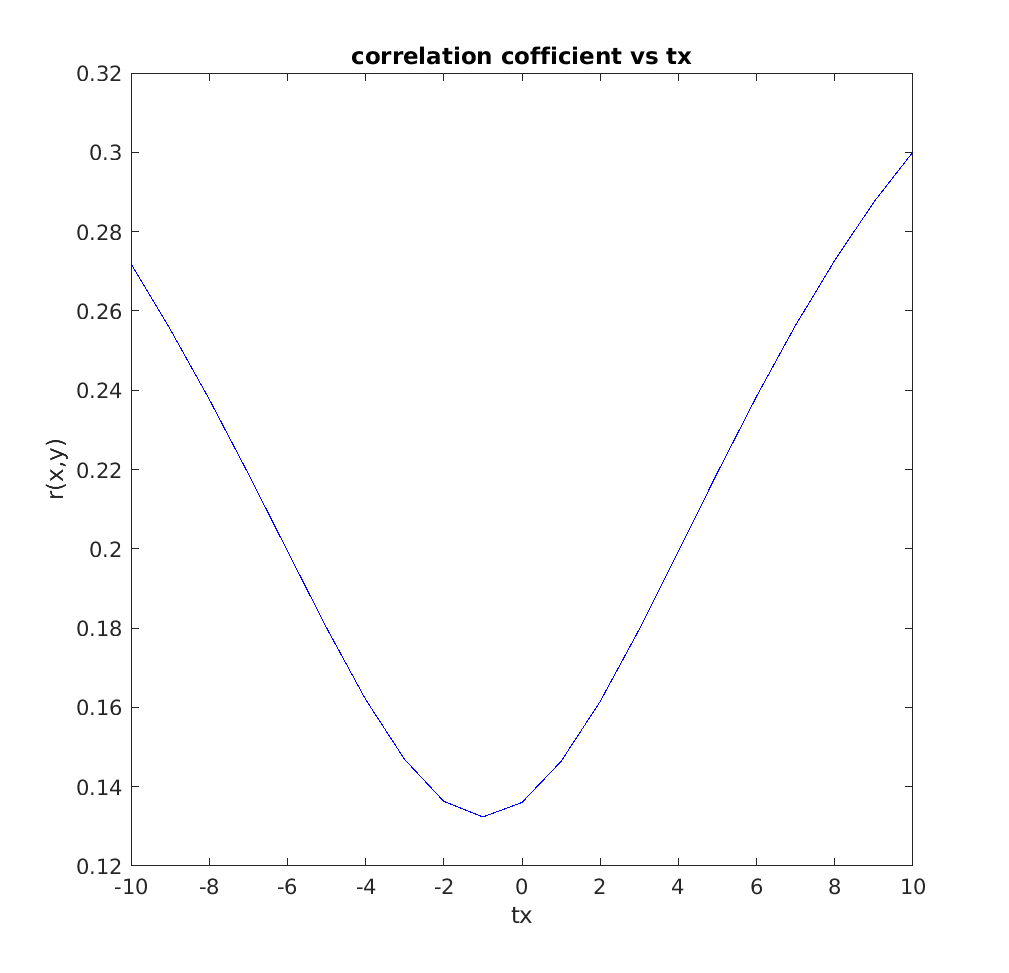
\includegraphics[width=\textwidth, height=\textheight, keepaspectratio]{cor_cof1.png}
\captionof {figure} {This plot correspond to T1.jpg and T2.jpg}
% \end{subfigure}

% \begin{subfigure}[b]{0.4\linewidth}
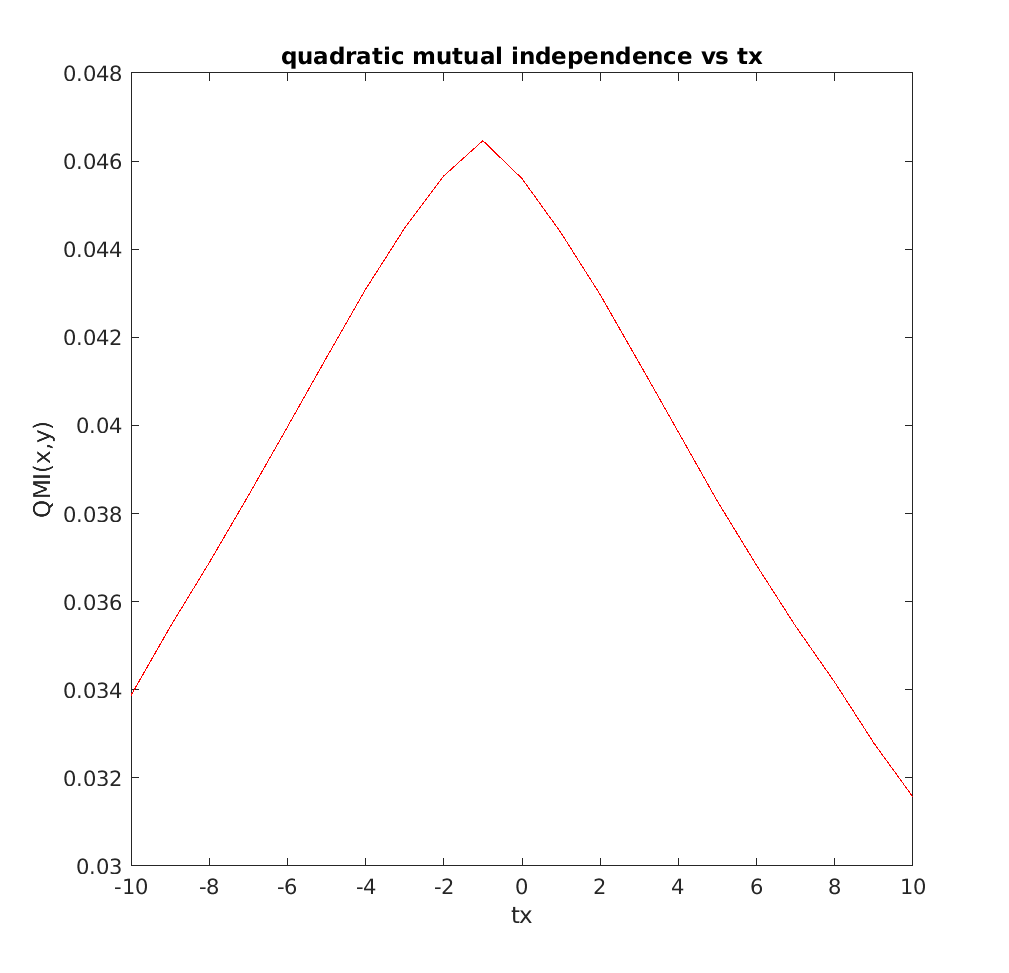
\includegraphics[width=\textwidth, height=\textheight, keepaspectratio]{quadMutInf1.png}
\captionof {figure}{This plot correspond to T1.jpg and T2.jpg}
% \end{subfigure}

% \begin{subfigure}[b]{0.4\linewidth}
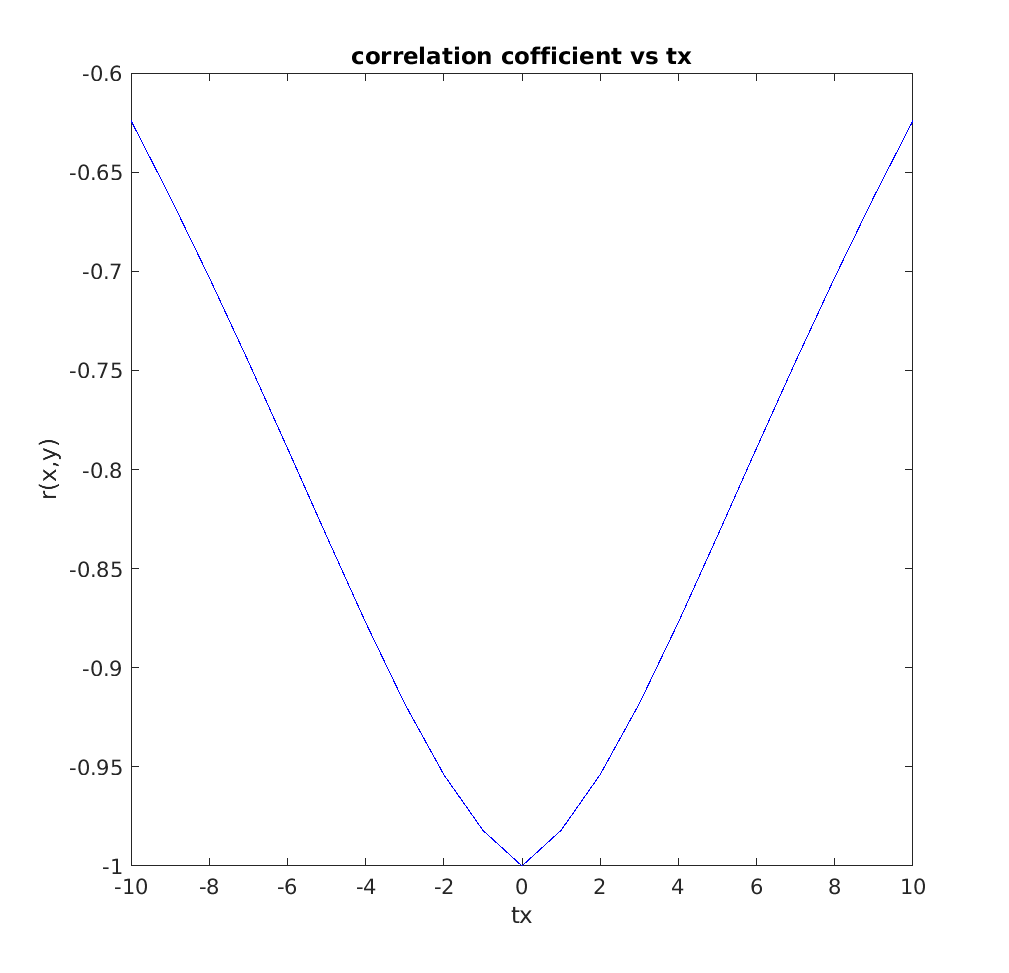
\includegraphics[width=\textwidth, height=\textheight, keepaspectratio]{cor_cof2.png}
\captionof {figure}{This plot correspond to T1.jpg and negative of T1.jpg}
% \end{subfigure}

% \begin{subfigure}[b]{0.4\linewidth}
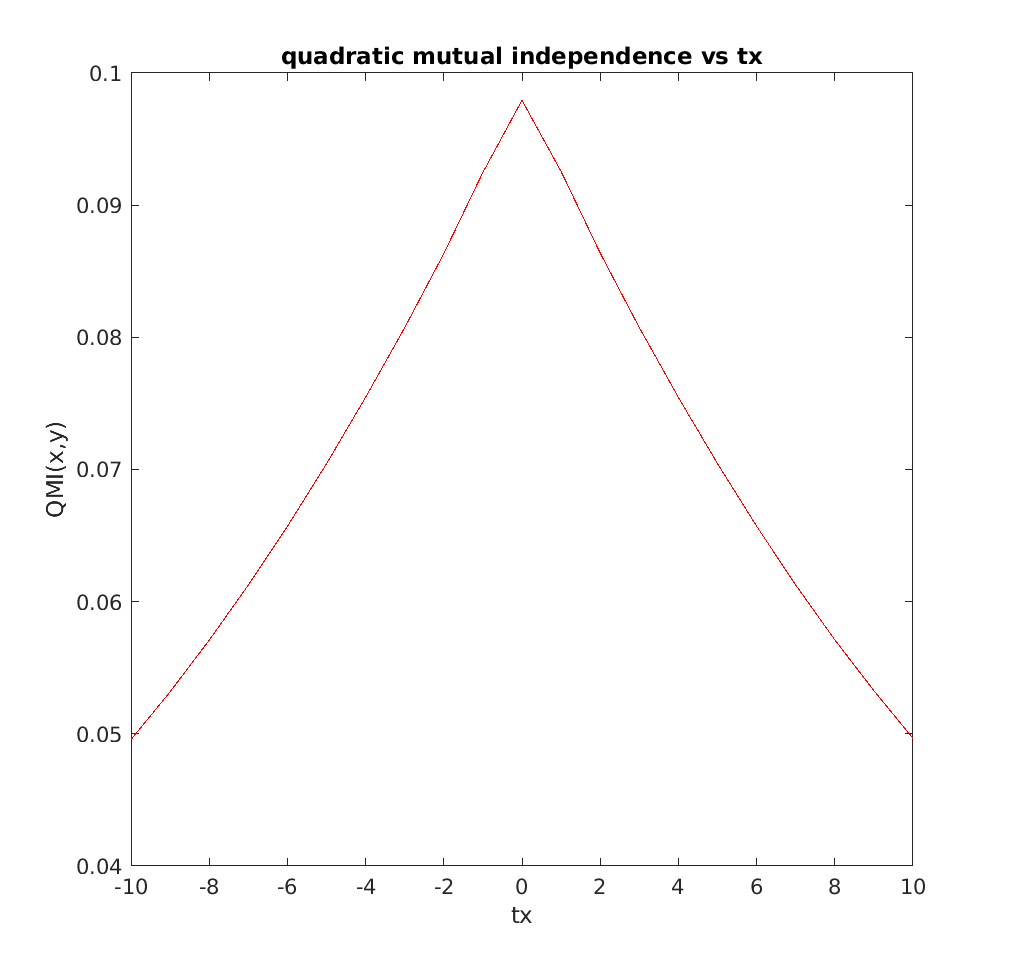
\includegraphics[width=\textwidth, height=\textheight, keepaspectratio]{quadMutInf2.png}
\captionof {figure}{This plot correspond to T1.jpg and negative of T1.jpg}
% \end{subfigure}

% \end{figure}

\par
\par
By observation we can see that correlation coefficient between the two images will be always postive, and it will minimum when the shift is equal to -1(that is one unit along negative x axis).By similar type of arguments we can say that QMI will attains it's maximum when the shift is equal to 1.We can say that correlation coefficient increases and QMI decreases when images are moved out of alignment as the point of minimum correlation coefficient and maximum QMI is somewhat close to no shift. \par
By observation we can see that correlation coefficient between the two images will be always negative, and it will minimum when the shift is equal to 0 and it will be equal to -1 as we can clearly see that the images are negative of each other.By similar type of arguments we can say that QMI will attains it's maximum when the shift is equal to 0.We can say that correlation coefficient increases and QMI decreases when images are moved out of alignment as the point of minimum correlation coefficient and maximum QMI is equal to no shift. \par

\newpage
\newpage



\section{Question 7}
\begin{figure} [h!]
    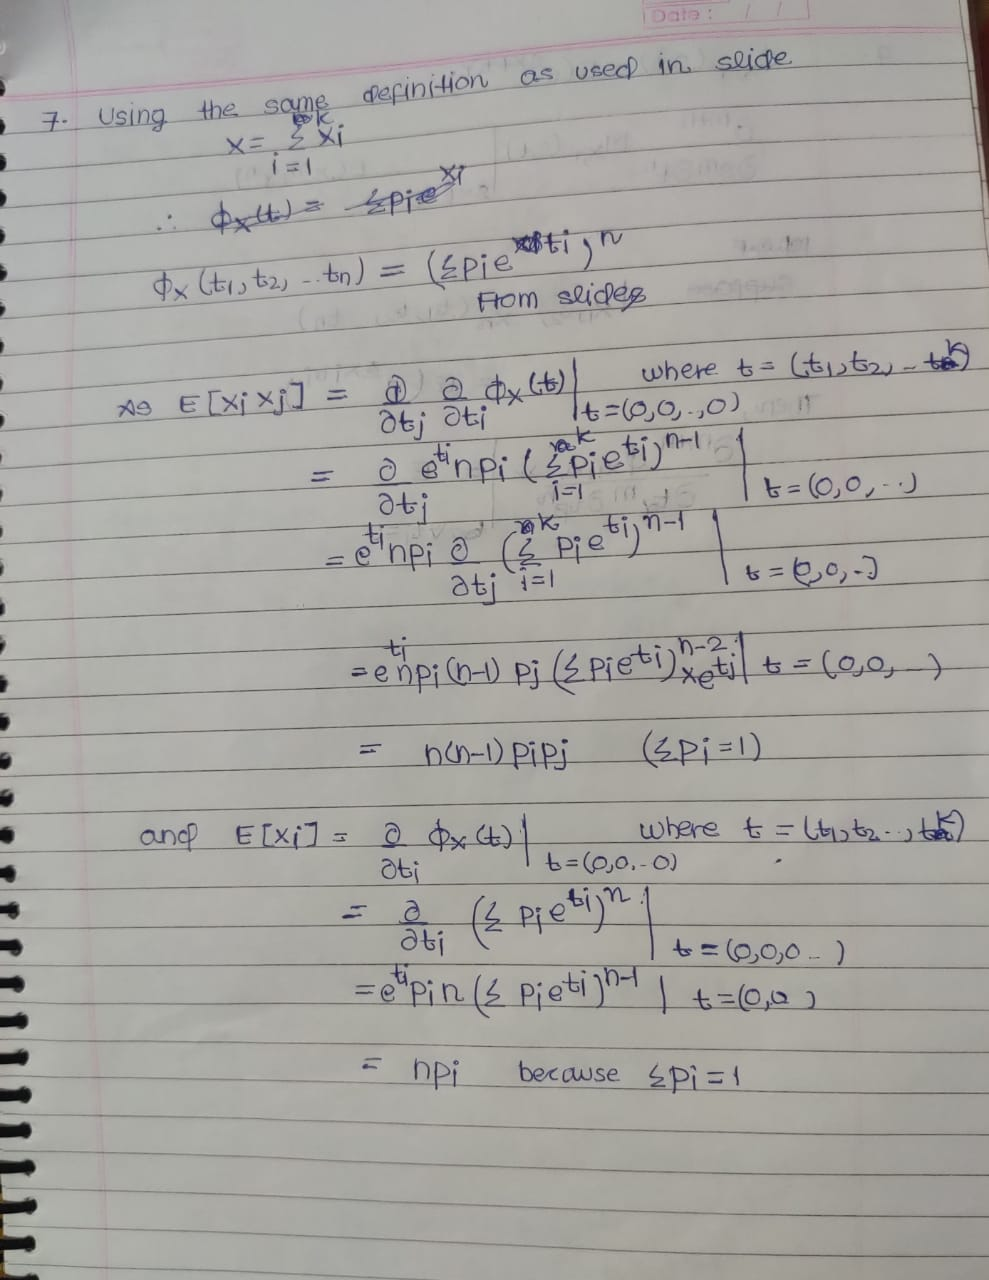
\includegraphics[width=\textwidth, height=\textheight, keepaspectratio]{7a.jpeg}\par

\end{figure}

\begin{figure}[h!]
    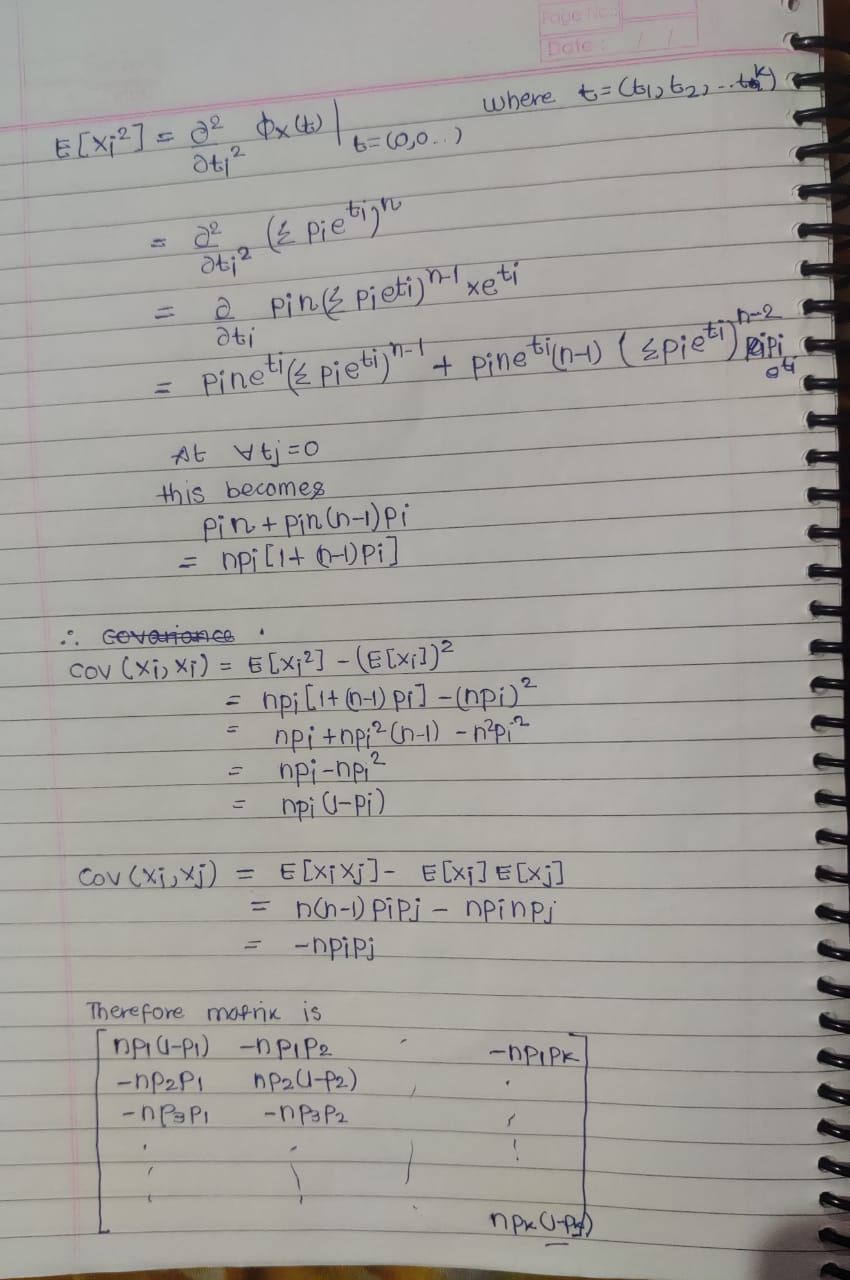
\includegraphics[width=\textwidth, height=\textheight, keepaspectratio]{7b.jpeg}\par
\end{figure}
\end{document}